\fullwidth{Use the following figure to fill in the blanks of the next four questions.}

\vspace*{-0.5\baselineskip}
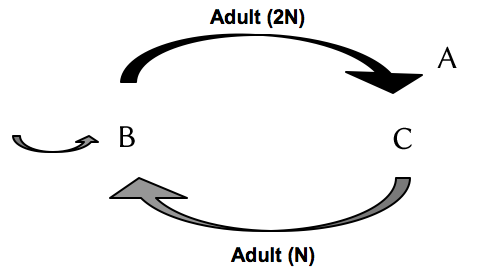
\includegraphics[width=0.5\textwidth]{life_cycleA}

\question
The process at A is \ifprintanswers\textbf{Meiosis}\else\rule{1.5in}{0.4pt}\fi


\vspace{1\baselineskip}

\question
The process (not the stage) that occurs at B is \ifprintanswers\textbf{Syngamy}\else\rule{1in}{0.4pt}\fi


\vspace{1\baselineskip}

\question
The stage at C (that results from A) is called \ifprintanswers\textbf{Spore}\else\rule{1in}{0.4pt}\fi


\vspace{1\baselineskip}

\question Which of the three (A, B or C) does not exist in the animal lifecycle. \ifprintanswers\textbf{C}\else\rule{1in}{0.4pt}\fi

\vspace*{2\baselineskip}

